\documentclass{article}
\usepackage[margin=2cm]{geometry}
\usepackage{graphicx}
\usepackage{subcaption}
\usepackage{tabu}
\usepackage{mathtools}
\title{COL783 Assignment 3}
\author{Lovish Madaan \\ \texttt{2015CS50286} \and Nikhil Goyal \\ \texttt{2015CS50287}}
\begin{document}
\maketitle
\section{Image Pyramid}
\begin{figure}[!ht]
\begin{subfigure}{.33\textwidth}
\centering
\includegraphics[width=.75\linewidth]{b.png}
\caption{Original Image}
\end{subfigure}
\begin{subfigure}{.33\textwidth}
\centering
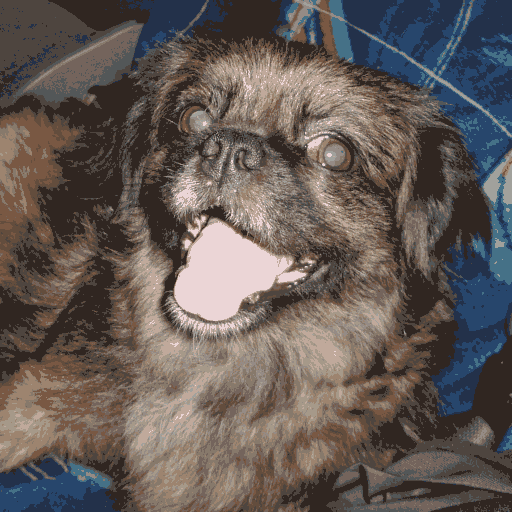
\includegraphics[width=.75\linewidth]{bquantized.png}
\caption{Median Cut Quantization}
\end{subfigure}
\begin{subfigure}{.33\textwidth}
\centering
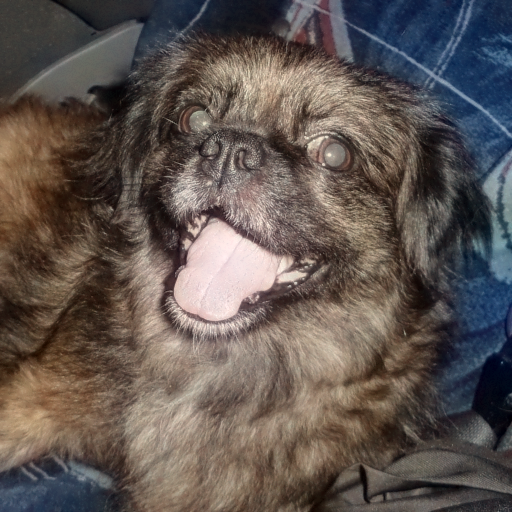
\includegraphics[width=.75\linewidth]{bcompressed.png}
\caption{Compressed Image}
\end{subfigure}
\end{figure}
Size of Compressed Image - $\frac{2}{9}$ of the original image $+$ Overhead.

\section{Image Inpainting}
\begin{figure}[!ht]
\begin{subfigure}{0.5\textwidth}
\centering
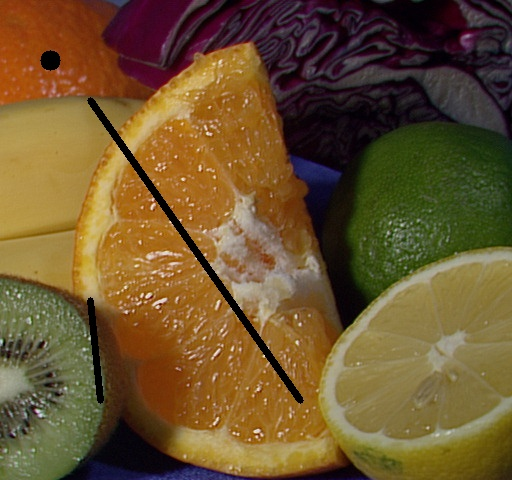
\includegraphics[width=0.75\linewidth]{fruits_damaged.jpg}
\caption{Damaged Image}
\end{subfigure}
\begin{subfigure}{0.5\textwidth}
\centering
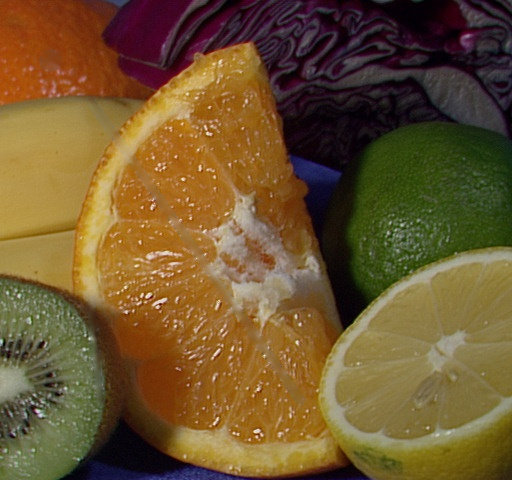
\includegraphics[width=0.75\linewidth]{fruits_painted.png}
\caption{Inpainted Image}
\end{subfigure}
\end{figure}
\clearpage
\section{Image Analogies}
\begin{figure}[!ht]
\begin{subfigure}{0.5\textwidth}
\centering
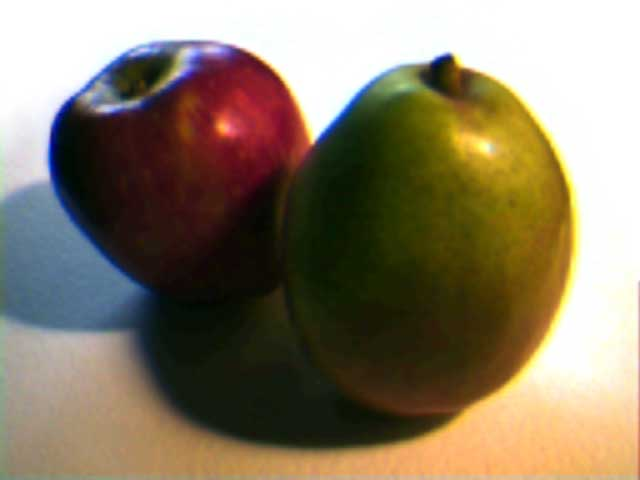
\includegraphics[width=0.75\linewidth]{watercolor-src.jpg}
\caption{A}
\end{subfigure}
\begin{subfigure}{0.5\textwidth}
\centering
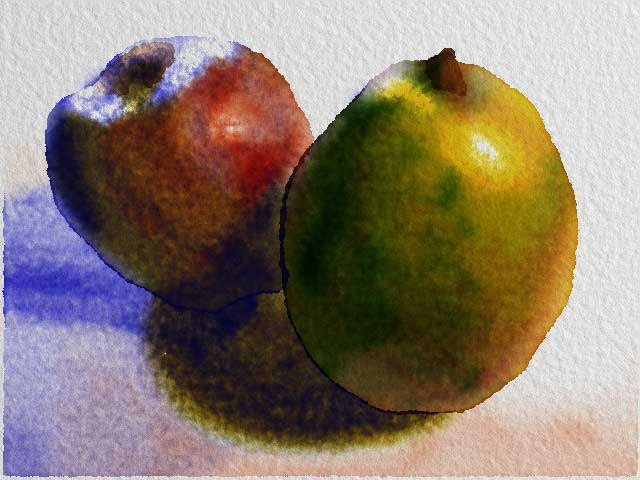
\includegraphics[width=0.75\linewidth]{watercolor.jpg}
\caption{A'}
\end{subfigure}
\end{figure}
\begin{figure}[!ht]
\begin{subfigure}{0.5\textwidth}
\centering
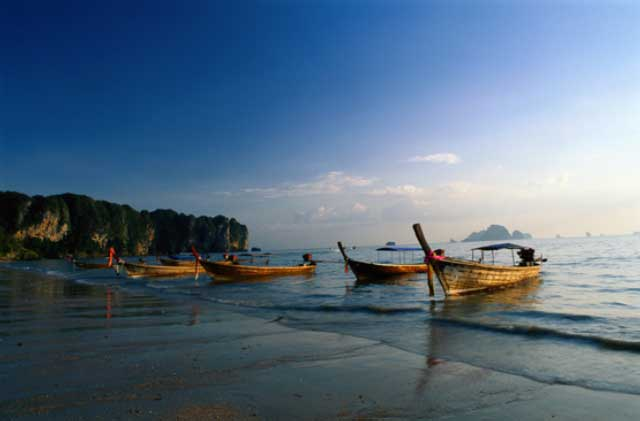
\includegraphics[width=0.75\linewidth]{boats.jpg}
\caption{B}
\end{subfigure}
\begin{subfigure}{0.5\textwidth}
\centering
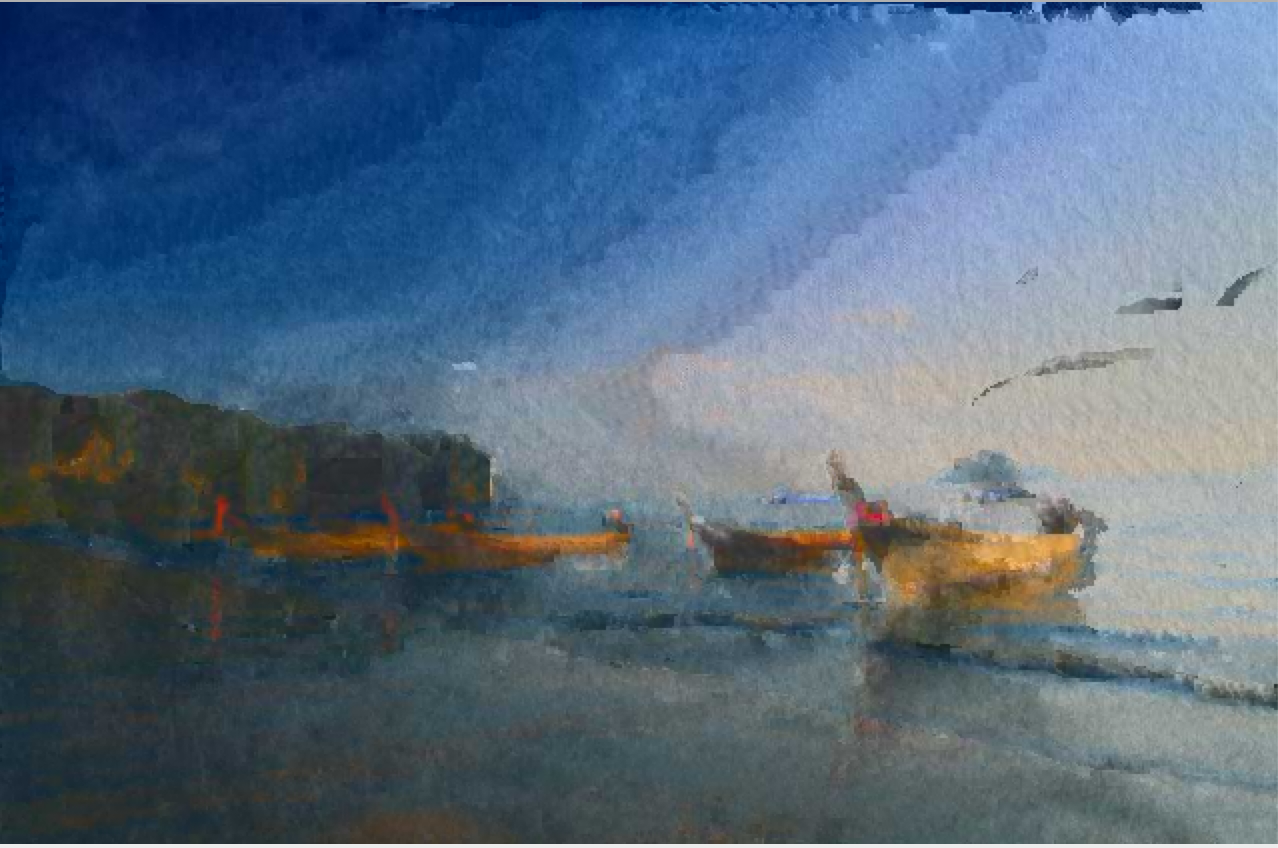
\includegraphics[width=0.75\linewidth]{B_prime.jpg}
\caption{B'}
\end{subfigure}
\end{figure}

\begin{figure}[!ht]
\begin{subfigure}{0.5\textwidth}
\centering
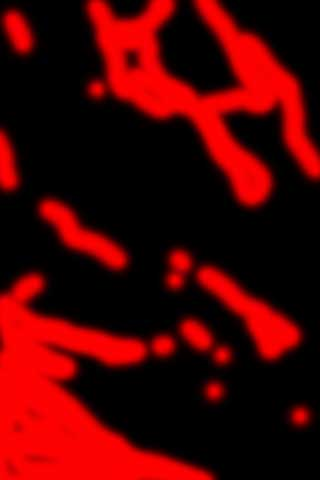
\includegraphics[width=0.75\linewidth]{waterfall-mask.jpg}
\caption{A}
\end{subfigure}
\begin{subfigure}{0.5\textwidth}
\centering
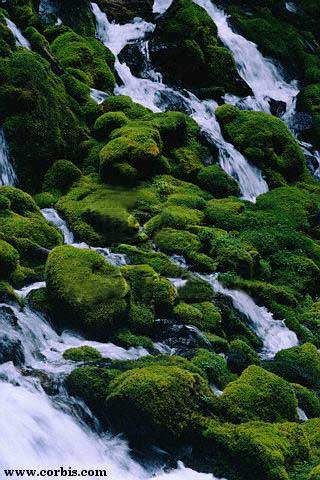
\includegraphics[width=0.75\linewidth]{waterfall.jpg}
\caption{A'}
\end{subfigure}
\end{figure}
\begin{figure}[!ht]
\begin{subfigure}{0.5\textwidth}
\centering

\includegraphics[width=0.75\linewidth]{waterfall-mask1.jpg}
\caption{B}
\end{subfigure}
\begin{subfigure}{0.5\textwidth}
\centering
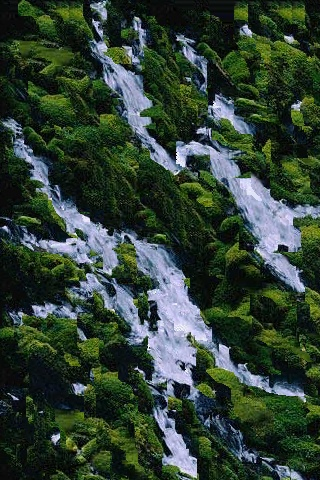
\includegraphics[width=0.75\linewidth]{B_prime2.jpg}
\caption{B'}
\end{subfigure}
\end{figure}
\end{document}